
\chapter{Array}

\section{What is an array?}

An Array is a collection of items.
The items are stored in neighboring (contiguous) memory locations.
Thus elements can be accessed randomly since each element in the array can be identified by an array index.

For example in the Figure \ref{fig:array-index}:

\begin{figure}[!ht]
  \centering
  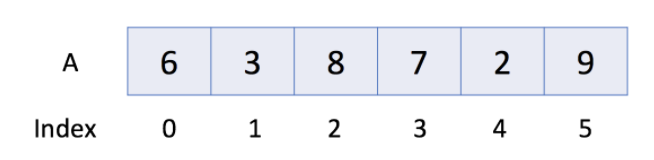
\includegraphics[width=0.7\textwidth]{pics/array-index}
  \caption{Array Index}
  \label{fig:array-index}
\end{figure}

In the above example, there are 6 elements in array A.
That is to say, the length of A is 6.
We can use A[0] to represent the first element in the array.
Therefore, A[0] = 6.
Similarly, A[1] = 3, A[2] = 8 and so on.

% \begin{tikzpicture}[>=latex]
% \matrix[mymat,anchor=west,row 2/.style={nodes=draw}]
% at (0,0) 
% (mat1)
% {
%   \\
% 2 & 1 & 3 & 2 & 1 \\
% };
% \end{tikzpicture}




\section{Capacity and length}

The capacity is the items it can hold at most.
It is specified when you create an array.

Length is the number of items it holds currently.


\section{Operations}

Array is a data structure, which means that it stores data in a specific format and supports certain operations on the data it stores.


There are three basic operations in array:
\begin{itemize}
\item insert
\item delete
\item search
\end{itemize}


\section{String}

A string is an array of characters.

\section{Examples}

\subsection{Diagonal traverse}

\begin{lstlisting}
#!/usr/bin/env python3
"""
@project: leetcode
@file: 20210303_diagonal_traverse
@author: mike
@time: 2021/3/3
 
@function:
Given a matrix of M x N elements (M rows, N columns),
return all elements of the matrix in diagonal order as shown in the below image.



Example:

Input:
[
 [ 1, 2, 3 ],
 [ 4, 5, 6 ],
 [ 7, 8, 9 ]
]

Output:  [1,2,4,7,5,3,6,8,9]

Explanation:



Note:

The total number of elements of the given matrix will not exceed 10,000.
"""
from typing import List
import collections


class Solution:
    def findDiagonalOrder(self, matrix: List[List[int]]) -> List[int]:
        dictionary = collections.defaultdict(list)
        for i in range(len(matrix)):
            for j in range(len(matrix[0])):
                dictionary[i + j].append(matrix[i][j])
        print(dictionary)

        maximum = len(dictionary)
        result = []
        for i in range(maximum):
            if i % 2 == 0:
                result.extend(list(reversed(dictionary[i])))
            else:
                result.extend(dictionary[i])
        return result


if __name__ == '__main__':
    solution = Solution()
    matrix = [
        [1, 2, 3],
        [4, 5, 6],
        [7, 8, 9]
    ]

    result = solution.findDiagonalOrder(matrix)
    print(result)

\end{lstlisting}


There are two manners to solve the problem:
\begin{enumerate}
\item based on the procedure
\item based on overview properties
\end{enumerate}






